\Introduction

Галактики не расположены случайным образом в пространстве. Они формируют собой особые структуры, 
такие как скопления и сверхскопления галактик. Эти структуры в свою очередь формируют собой цепи, 
или так называемые "нити".\\

\begin{figure}
    \center{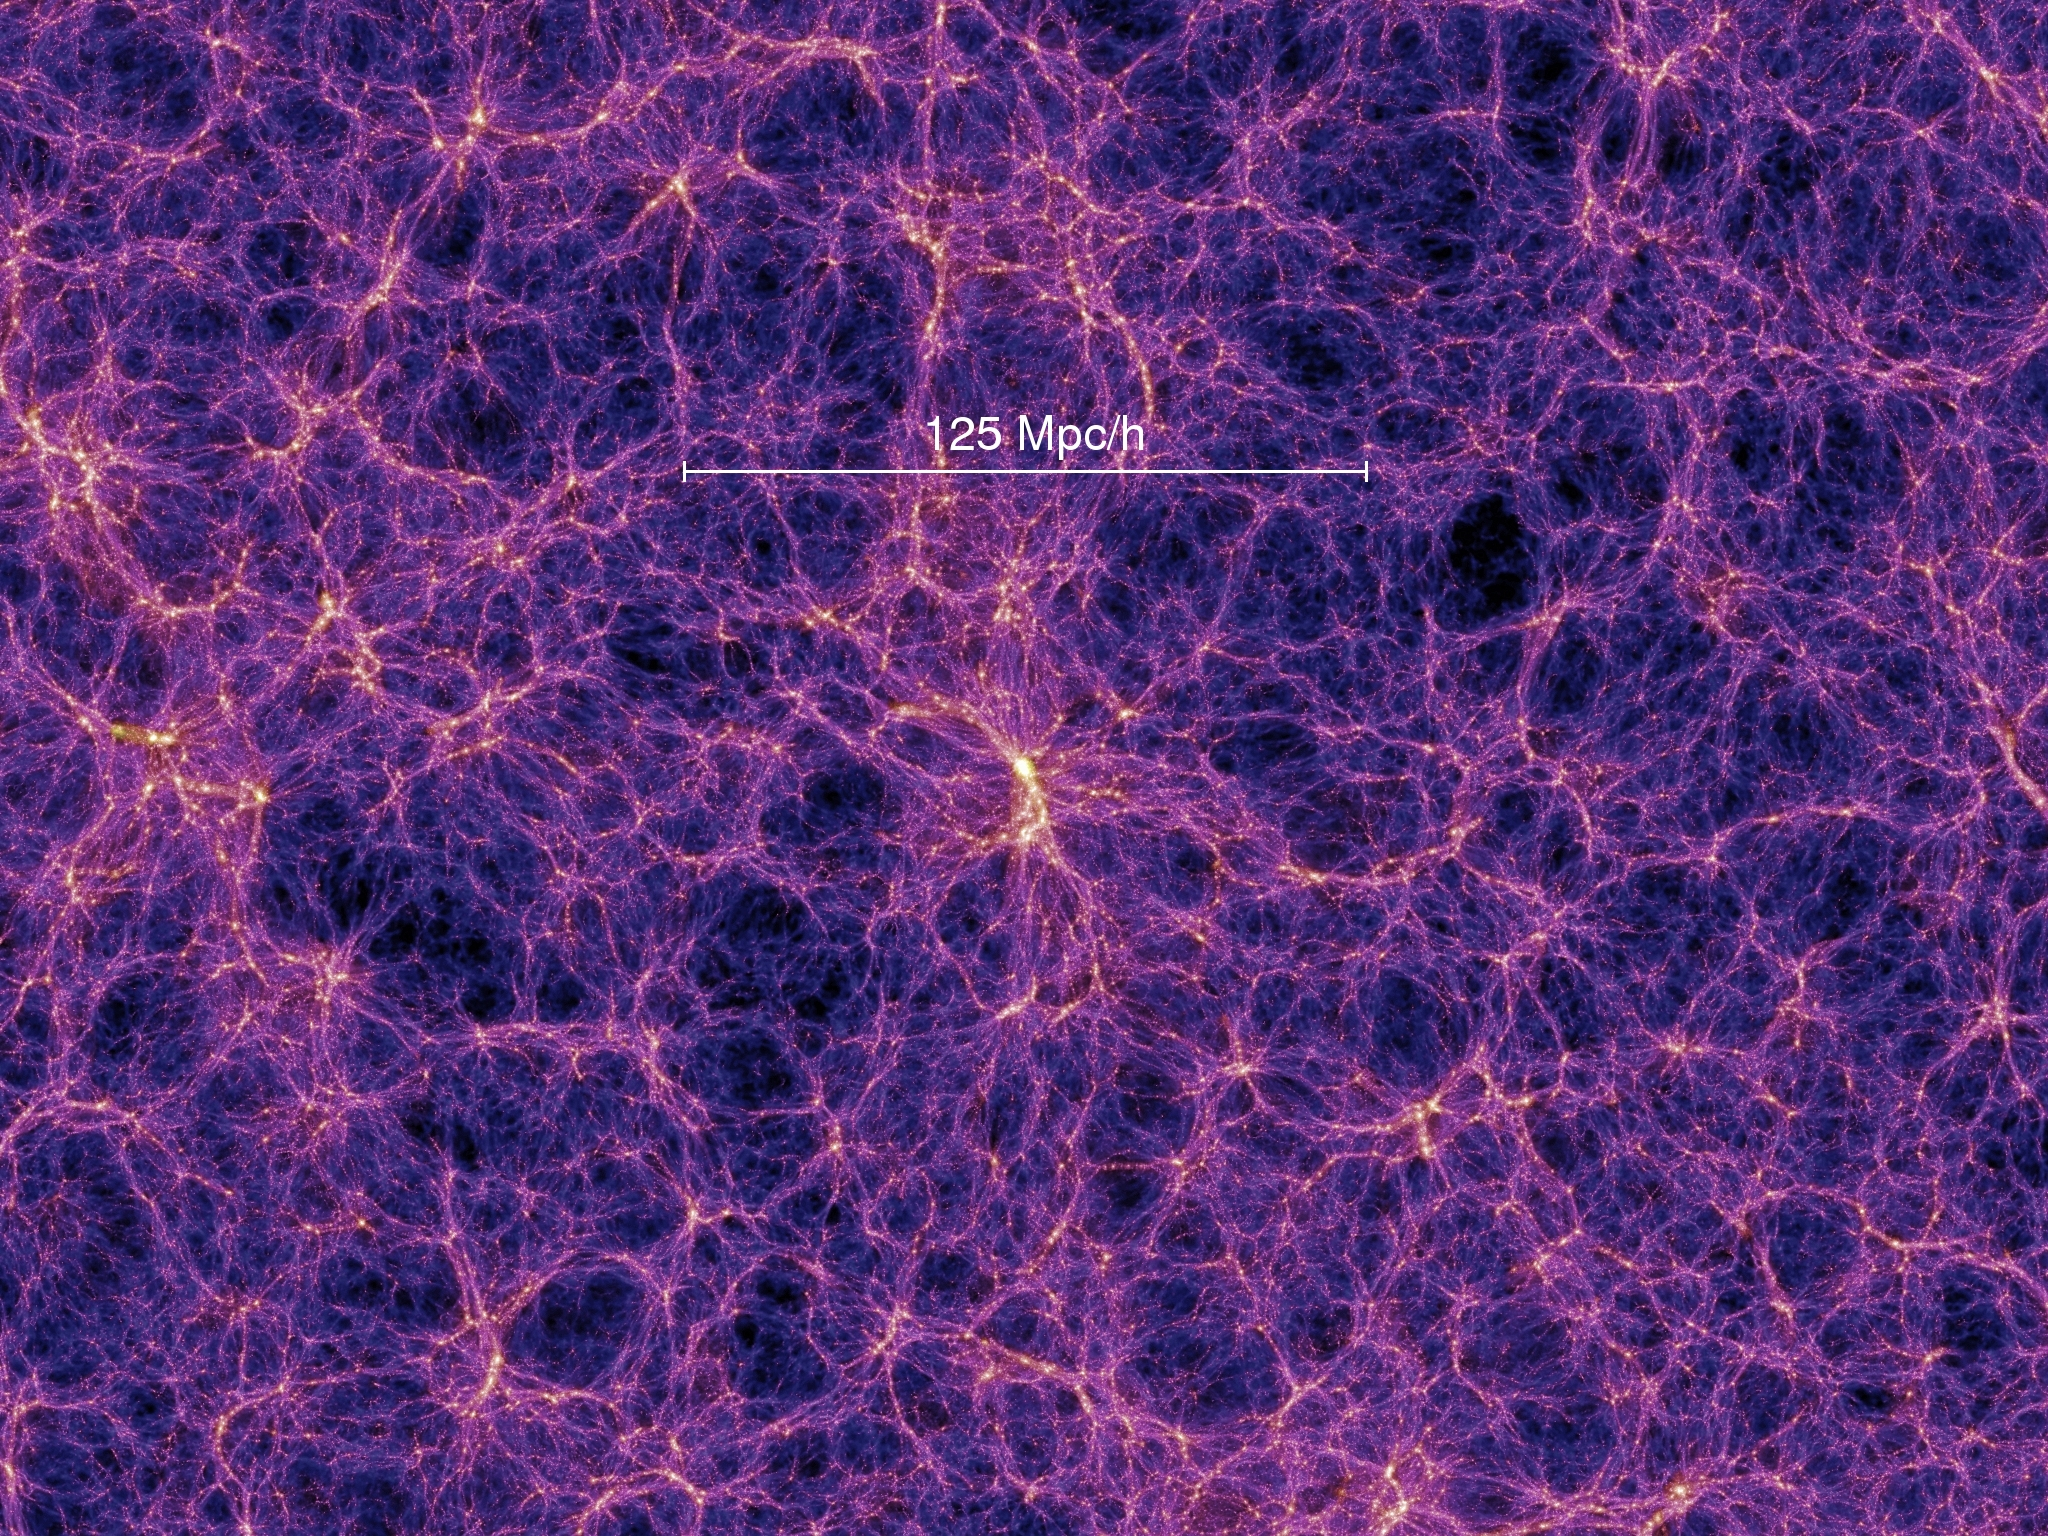
\includegraphics[width=0.6\linewidth]{millennium}}
    \caption{Моделирование «Милленниум» — N-частичное моделирование, проведённое Консорциумом 
        Девы с целью изучения формирования крупномасштабной структуры Вселенной в стандартной
        космологической модели.}
\end{figure}

Скопления галактик представляют большой интерес для исследования, так как их свойства сильно зависят 
от космологических параметров. Изучая их свойства, можно делать выводы о структуре обозримой части 
Вселенной.\\

Сама по себе крупномасштабная структура Вселенной имеет объяснение. При появлении Вселенной 
возмущения волн плотности средних и больших масштабов при совпадении пиков образовали сверхскопления,
в то время как сопадения фаз низкой плотности образовали войды - огромные пространства между нитями 
скоплений, в которых почти отсутствуют галактики и скопления. Таким образом, зная расположение и 
параметры большого количества скоплений, можно сделать выводы о том, как развивалась Вселенная на 
ранних этапах.\\

